This chapter explains the characteristics of the launch and space segments of the mission. Section \ref{frLS} describes the three main parts in bringing the swarm into the orbit: launch vehicle, launch location and orbit insertion. Section \ref{frSS} discusses all the aspects of the constellation and its configuration, and delves into estimations of $\Delta$V and needed propellant. Finally, section \ref{frSEaS} deals with the hazardous space environment and ways of protecting the satellites against it. 

\section{Launch Segment}
\label{frLS}

The launch segment of the mission includes the selection of the launch vehicle, the launch location and the procedure of inserting the satellites into their respective orbits. The following subsections discuss all of these aspects. 

\subsection{Launch Vehicle}
\label{frLSLV}

The costs of launch vary greatly between different vehicles. Table \ref{table:vehicleCosts} on page \pageref{table:vehicleCosts} lists approximate total launch costs of respective platforms. For consistency, the prices are given in Fiscal Year 2000 dollars.
\begin{table}[h]
\begin{centering}
\begin{tabular}{llr}
\toprule
Platform & Operator & Price (FY00M\$) \\
\hline \hline
Ariane V  & ESA & 97.96 \\
Soyuz   & Starsem or Arianespace&  8.16 - 22.1 \\
Vega   & European and Italian SA  & 15.1 \\
Falcon 1E  & SPACEX  & 8.89 \\
PSLV & ISRO & 13.88 - 16.33 \\
Rokot & Eurokot & 9.8 - 11.4 \\
\bottomrule
\end{tabular}
\caption{Estimated price comparison of different launch vehicles. \emph{(Source: various.)}}
\label{table:vehicleCosts}
\end{centering}
\end{table}

Based on the information  in the above table it is possible to single out a few platforms which will be affordable for the purpose of this feasibility study. The values represent the total launch segment costs. The Ariane V launcher is the most expensive option by far and would push the budget quite heavily, with an estimated cost of launch almost half of the total budget. However the payload capabilities of the Ariane V launcher far outweigh that of all other platforms, thus making it possible for a combined launch with other satellites, leading to shared costs. This however could jeopardize the mission in the sense that it becomes secondary priority. If that happens, the constellation would have higher requirements for orbit acquisition: an extra booster stage or higher onboard fuel capacity for the altitude and/or plane shift, which is not feasible. The Ariane V is therefore an unsuitable platform for this project. 

The rest of the launchers can be analyzed with respect to reliability. All of the launch vehicles have been tested, with the exception of the Vega system, which is yet to make its maiden flight. The Vega is therefore not suitable for the analysis at this time. It is for this reason that the project will no longer consider this system at all.  However, better data should be available in the near future which should allow for the Vega platform to be reevaluated.

The same goes for the Falcon 1e. The launcher is an incremental improvement on the Falcon 1, of which only the last two launches out of five were successful. This technology is not proven enough for the purpose of the mission.

Table \ref{table:LVreliability} on page \pageref{table:LVreliability} shows some reliability statistics for the remaining 3 vehicles.

\begin{table}[h]
\begin{centering}
\begin{tabular}{lcccp{5cm}}
\toprule
Platform & Total No. of Launches & Total Failures & Reliability & No. of Successful Launches Since Last Failure  \\
\hline \hline
Soyuz   & 1754  &  88 & 95\% & 57 \\
PSLV & 16 & 1 & 94\% & 15 \\
Rokot & 17& 2 & 88\% & 6 \\
\bottomrule
\end{tabular}
\caption{Reliability figures for several launch vehicles. \emph{(Source: various.)} }
\label{table:LVreliability}
\end{centering}
\end{table}

The Soyuz launch vehicle presents itself as the most reliable platform, with a track record that far surpassed all other options. This launch vehicle will be the one considered for this project. In the next section, its payload capabilities are discussed.

\subsubsection{Soyuz LV Payload Capability Analysis}
\label{frLVPCA}

There is a large selection of Soyuz vehicles available for consideration. For the purpose of this project, the newest modification - Soyuz-ST will be used. This vehicle is part of the Soyuz-2 family, which are technologically superior to the older Soyuz-U and U2 launchers. An illustration and technical parameters of the Soyuz-ST can be found in Appendix \ref{appa} on page \pageref{appa} \cite{soyuzman}.

An estimation of mass performance for the launch vehicle can be seen in figure \ref{fig:massperformance} on page \pageref{fig:massperformance}.

\begin{figure}[ht]
\centering
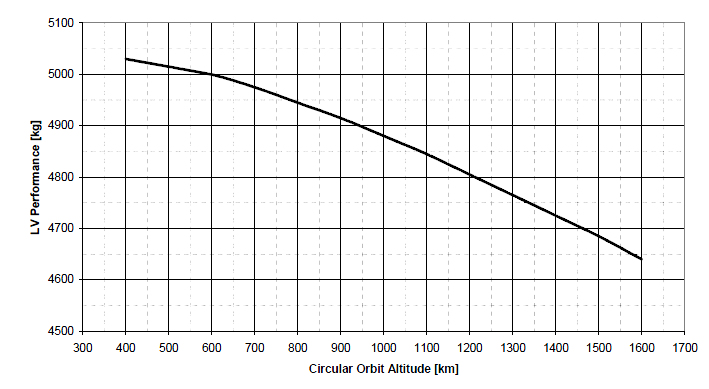
\includegraphics[width=0.6\textwidth, angle=0]{chapters/img/lvmass.png}
\caption{Mass performance of the Soyuz-ST for circular orbits. \emph{(Source: \cite{soyuzman}.})}
\label{fig:massperformance}
\end{figure}

The payload mass data provided in \cite{soyuzman} is estimated, yet is good enough to have a reasonable idea about the maximum mass. The Soyuz-ST is able to launch roughly a maximum of 5000 kg into a 500 km orbit. This is well above the design mass of the formation thus will allow for further considerations of joint launches (as long as the swarm mission is considered to be the primary payload) and thus spread launch costs. 

The available volume in the Soyuz-ST Fairing can be seen in figure \ref{fig:soyuzvol} on page \pageref{fig:soyuzvol}.

\begin{figure}[ht!]
\centering
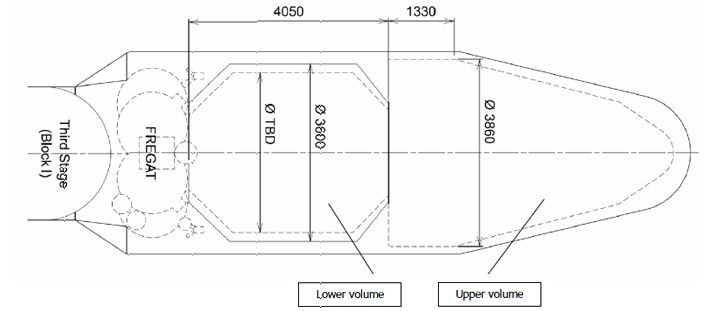
\includegraphics[width = 0.8\textwidth, angle=0]{chapters/img/soyuzvolRotated.png}
\caption{Fairing volume of the Soyuz-ST launch vehicle. Here shown in dual launch carrying configuration.\emph{ Source: \cite{soyuzman}.}}
\label{fig:soyuzvol}
\end{figure} 

The dimensions of the fairing are visibly too large and there is no possibility of using a different one, however that leaves a lot of possibilities for different designs of release adapters to adapt to the unique sequence of separation upon orbit injection. Again, the possibility of taking other small satellites along on the same launch arises. The dual launch configuration shown in the previous figure is the one being considered for the launch.

The choice of the Soyuz brings forth one more advantage: the use of a unique orbit insertion booster, the Fregat. This final stage will allow for minimization of fuel on the satellite as all orbit insertion maneuvers can be done using the Fregat. The Fregat stage has been designed to handle 20 individual burns.

\subsubsection{Vibrational Analysis}
\label{frLVCA}
The launch is a critical part of the mission for the survival of the payload. It is during this period that the payload will experience the most severe loads. In this section the origin and magnitude of these loads will be discussed, as well as their impact on the payload. The main loads are the quasi-static loads, shock loads, sinusoidal loads, random vibrations and acoustic vibrations.

Quasi-static loads are caused by the engine thrust. The acceleration will increase steadily as the amount of fuel becomes less. Peaks are reached when the engines run out of fuel and stop giving thrust. The ignition of a stage also results in a peak load. These loads are all in the longitudinal direction. There are also quasi-static loads in the lateral direction caused by ground maneuvers and wind gusts. These kind of loads are expressed as load factors. The maximum load factors for the Soyuz launcher are $+1,5/-5\ g$ in longitudinal direction and $+1,8/-1,8\ g$ in lateral direction.

Shock loads are high acceleration loads over a short period of time. They are mostly the result of separation events such as the separation of the boosters, different stages of the launcher and the payload fairing. They also occur with the deployment of appendages such as the solar panels. The shock response spectrum of some launchers is given in figure \ref{fig:SRS} on page \pageref{fig:SRS}.

\begin{figure}[ht!]
\centering
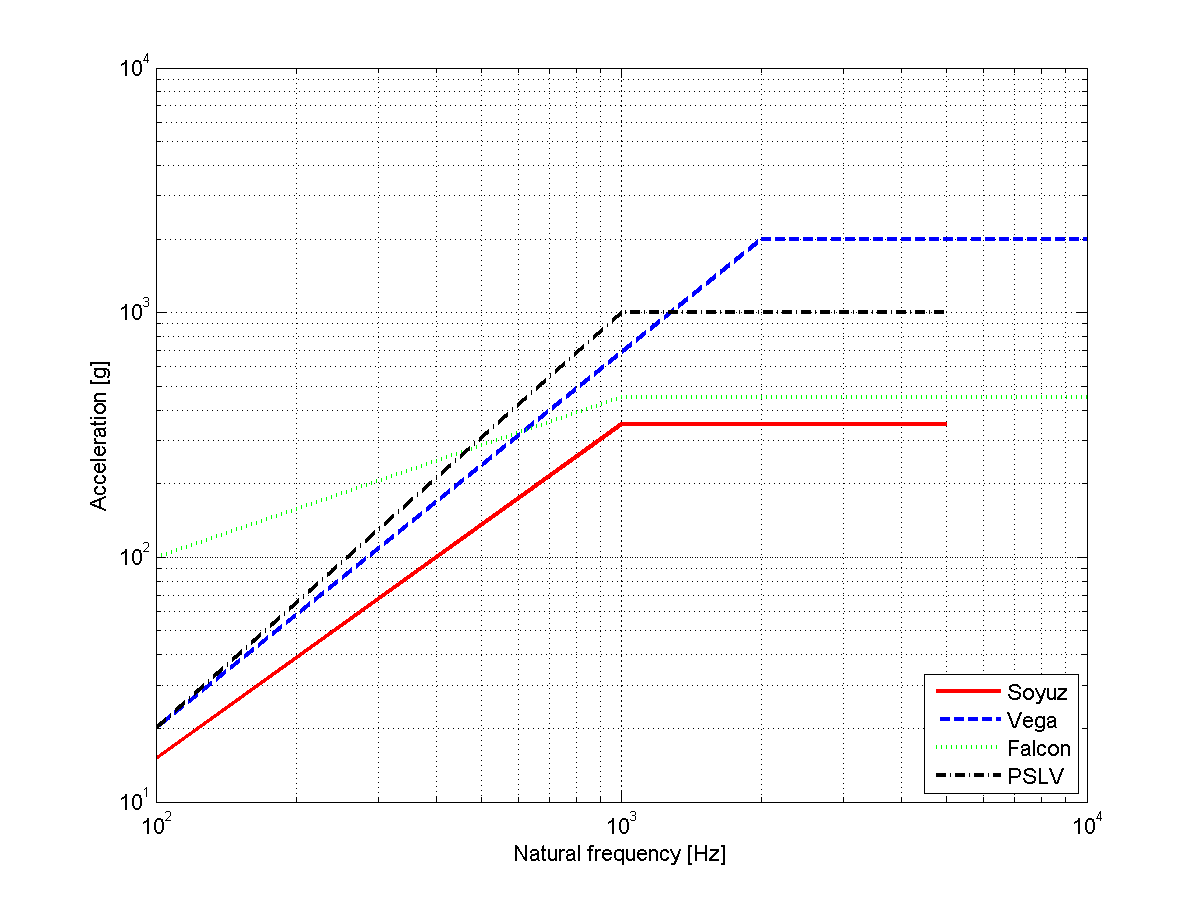
\includegraphics[width=0.5\textwidth, angle=0]{chapters/img/Shock_Loads_Acceleration.png}
\caption{Launch shock response spectrum as a function of payload natural frequency.}
\label{fig:SRS}
\end{figure}

The release of the payload from the adapter also causes a shock load, but with smaller accelerations than during launch. Ruag space has developed a low-shock release mechanism (\ac{CBOD}). The \acs{CBOD}'s shock response spectrum is shown in figure \ref{fig:CBOD_SRS} on page \pageref{fig:CBOD_SRS}.

\begin{figure}[ht!]
\centering
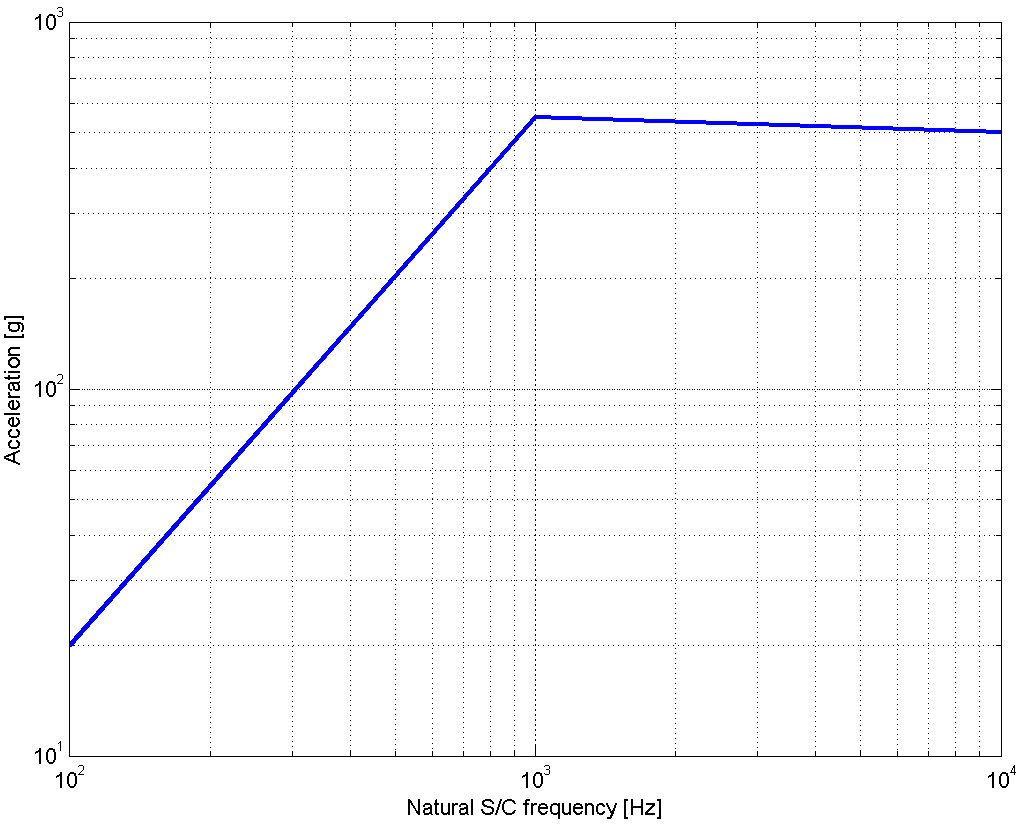
\includegraphics[width=0.5\textwidth, angle=0]{chapters/img/CBOD_release_acceleration.png}
\caption{Shock response spectrum of the \acs{CBOD} release mechanism.}
\label{fig:CBOD_SRS}
\end{figure}

Another critical load source are random vibrations. For the Soyuz launcher, only random vibrations between 20 and 100 Hz need to be taken in to account because higher frequencies are covered by acoustic vibrations. Random vibrations are caused by the propulsion system and the vibro-acoustic response of the neighboring structures. Table \ref{tab:random_vibr} on page \pageref{tab:random_vibr} gives the power spectral density, root mean square vibration and the duration of the sources for each part of the launch.

\begin{table}[H!]
\centering
\begin{tabular}{ccccc}
\toprule
 Event & \multicolumn{2}{c}{PSD $[g^2/Hz]$} & $G_{rms} [g]$ & Duration [s] \\
 \midrule
 Frequency band [Hz] & 20 - 50 & 50 - 100 & & \\
 \midrule
 First stage flight & 0.005 & 0.005 - 0.01 & 4.94 & 120 \\
 Second stage flight & 0.0025 & 0.0025 & 3.31 & 480 \\
 Third stage flight & 0.0025 & 0.005 & 3.31 & 480 \\
 Fregat flight & 0.002 & 0.002 & 1.63 & 875 \\
 \bottomrule
 \end{tabular}
 \caption{Soyuz maximum random vibrations \emph{ Source: \cite{soyuzman}.}}
\label{tab:random_vibr}
\end{table}

Acoustic vibrations are higher than random vibrations, up to 10 000 Hz. The main sources are the acoustic noise that radiates from the engines and from aerodynamic turbulence when the launcher passes through the trans-sonic part of the flight. During ground operations the venting system also produces noise. For the Soyuz launcher, this does not exceed 94 dB. Apart from the lift-off and the trans-sonic part of the flight, the acoustic vibrations are rather low. The structures that are affected the most by acoustic loads are structures with a low mass and high surface area, such as solar panels and skins sections. Table \ref{tab:acoustic_vibr} gives the acoustic noise spectrum under the fairing.

\begin{table}[H!]
\centering
\begin{tabular}{cc}
\toprule
Octave Center & Flight limit level [dB]\\
Frequency [Hz] & (reference: 0 dB = 2 X $10^{-5} Pa$ ) \\
\midrule
31.5 & 125\\
63 & 132 \\
125 & 134 \\
250 & 136 \\
500 & 134 \\
1000 & 125 \\
2000 & 121 \\
\bottomrule
 \end{tabular}
 \caption{Soyuz acoustic noise spectrum \emph{ Source: \cite{soyuzman}.}}
\label{tab:acoustic_vibr}
\end{table}

Sinusoidal loads occur mainly during the atmospheric flight. They are caused by lift off, bending of the rocket motors, aerodynamic buffeting and oscillations in the propulsion system. To avoid these kind of vibrations, the payload must be constructed in such a way that the payload's natural frequencies will not be close to those of the launcher. This will avoid resonance and thus the payload will experience much lower loads. For the Soyuz launcher it is required that the natural frequencies of the payload will be higher than 15 Hz in lateral direction and higher than 35 Hz in longitudinal direction. 

\subsection{Launch Site}
\label{frLSLS}

The selection of the launch site relies on several factors:

\begin{itemize}
	\item Availability of attainable inclinations from launch.
	\item Compatibility with the launch vehicle.
	\item Accessibility and cost.
	\item Security and political reasons. 
\end{itemize}

The first factor is crucial. It is paramount that the satellites are injected into their final inclinations at launch and do not have to perform any inclination change maneuvers, which require a substantial amount of $\Delta$V. With this in mind choosing a launch site closer to the equator is necessary. Launch sites at higher latitudes would need to sacrifice velocity and thus payload mass because of their location. Table \ref{table:launchtable} on page \pageref{table:launchtable} shows a number of possible launch sites and their locations \cite{larson}. The list contains only the sites compatible with the Soyuz-ST launch vehicle. Furthermore, in figure \ref{fig:launchsites} on page \pageref{fig:launchsites}, the same sites are indicated with their respective authorized inclination ranges.

\begin{table}[ht!]
\begin{centering}
\begin{tabular}{llp{2cm}p{2cm}}
\toprule
Launch Site & Operator & Latitude (deg min) & Longitude (deg min) \\
\hline \hline
Baikonur LC-31/6  & Russia (Starsem) & 45 54 N & 63 18 E \\
Plesetsk LC-43  & Russia (Starsem)   &  62 48 N & 40 24 E \\
Guiana Space Centre  ELS  & CNES/Arianespace  & 5 18 N & 52 50 W \\
\bottomrule
\end{tabular}
\caption{Available launch sites for the Soyuz-ST. \emph{(Source: \cite{larson}.)}}
\label{table:launchtable}
\end{centering}
\end{table}  

\begin{figure}[ht!]
\centering
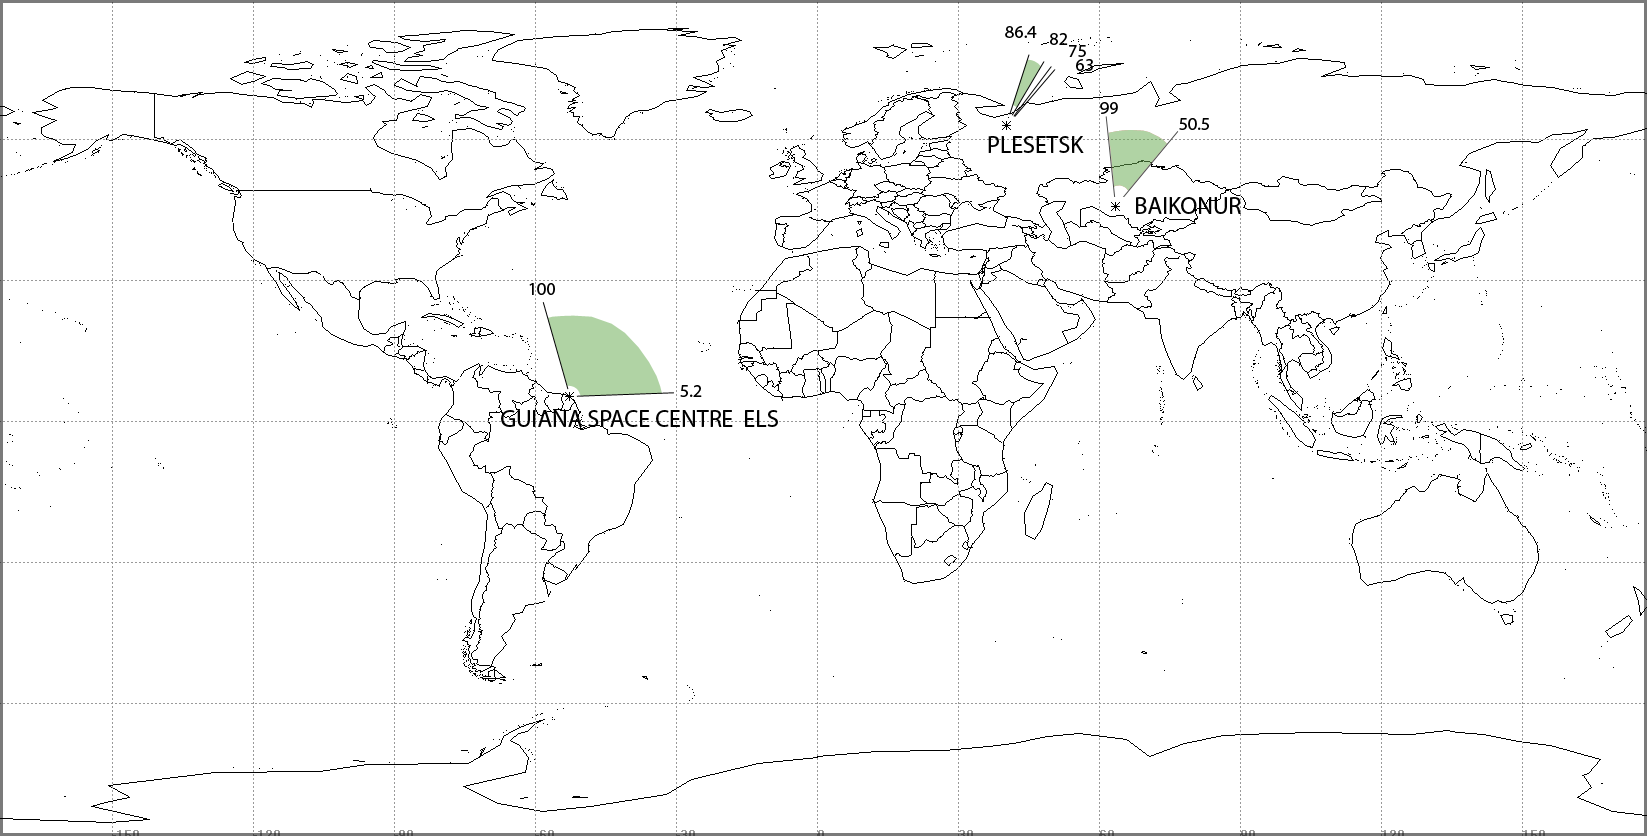
\includegraphics[width=1.0\textwidth, angle=0]{chapters/img/launchsites.png}
\caption{Launch site locations and allowable inclinations for the Soyuz-ST. \emph{(Sources: \cite{constDesign} and \cite{rockotman}.)} }
\label{fig:launchsites}
\end{figure}

Even though all the sites in table \ref{table:launchtable} allow inclinations of 85 degrees, it is still preferable to select a site closer to the equator in order to utilize the full effect of Earth's rotation and lower the launch costs. With this in mind, the Guyana Space Centre is selected to be the preferable location for launch.

The \ac{ELS} in Kourou, Guyana is currently being finalized and should accommodate its first Soyuz launch in 2010 \cite{arianesoyuz}.

A typical launch profile of the Soyuz launch vehicle from Kourou is shown in figure \ref{fig:launch} on page \pageref{fig:launch}. The first three stages of the vehicle are used to propel the payload and the Fregat booster in to a circular orbit at around 200 km. After separation (stage 6 on the figure), the Fregat initiates the first orbit injection burn to bring the satellites to the appropriate orbits.

\begin{figure}[ht]
\centering
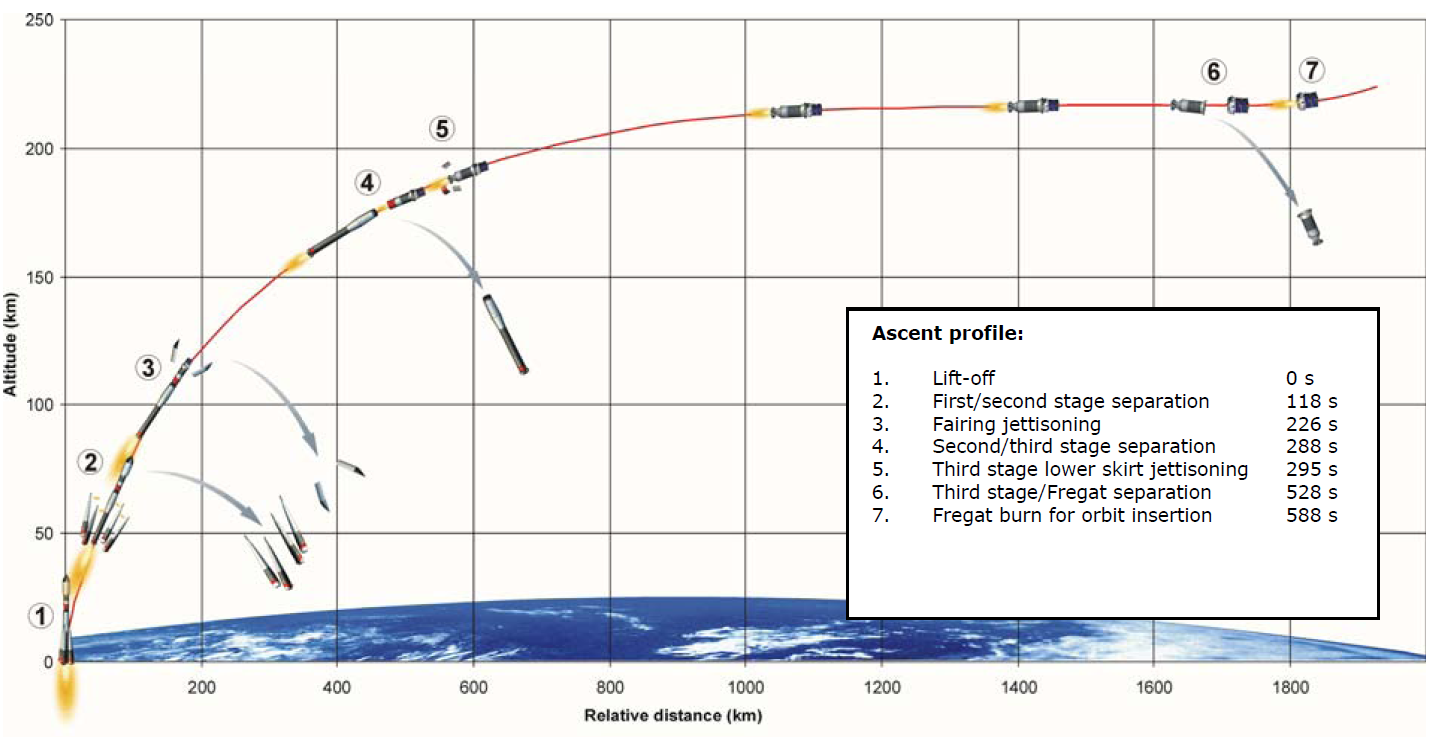
\includegraphics[width=1.0\textwidth, angle=0]{chapters/img/launchprofile.png}
\caption{Launch profile of the Soyuz LV from Kourou. \emph{(Sources: \cite{soyuzman}.)} }
\label{fig:launch}
\end{figure}

With this information it is possible to further calculate some important launch parameters:

\begin{itemize}
	\item The inertial velocity of the launch site is given by:
	
	\begin{equation} 
 		V_L = (464.5) cos L 
	\end{equation}
	
	where $L$ is the site latitude. For the case of Kourou the inertial velocity is 462.51 m/s.
	\item The launch azimuth in the inertial frame of reference is given by:
	
	\begin{equation} 
 		A_{Z_I} = arcsin(\frac{cos i}{cos L})
	\end{equation}
	
	and is equal to 5.022 degrees for this launch.
	\item The launch azimuth corrected for the Earth's rotation, is given by:
	
	\begin{equation} 
 		A_Z = arctan(\frac{V_0sinA_{Z_I}-V_{eq}cosL}{V_0cosA_{Z_I}})
	\end{equation}
	
	where $V_0$ is the orbital velocity reached by the launcher before separation and the first burn of the Fregat upper stage (see above, around 7.784 km/s), $V_{eq}$ is the velocity of the Earth's rotation at the equator - 464.5 m/s. Thus the corrected launch azimuth becomes 1.61 degrees. 
	
	\item The required launch velocity is calculated to be 7.76 km/s which means that due to Earth's rotation 26.8 m/s are saved.
\end{itemize}

Furthermore the region is politically stable and the launch site is under the protection from the French government and other security forces. All safety procedures are kept to the highest of standards and the spaceport is easily accessible by air or sea (Source: \cite{soyuzman}).

\subsection{Orbit Insertion}
\label{frLSOI}

The orbit insertion is separated into two distinct stages: primary orbits and secondary orbits. The primary orbits are located at an altitude of 500 km and contain the emitter and four initial receivers. The secondary orbits are located at a slightly different altitude of 525 km and contain the auxiliary receivers intended for replenishment.

The configuration of the primary orbits is discussed in section \ref{frSSSC} and an image of the formation can be seen in figure \ref{fig:confmax} on page \pageref{fig:confmax}. The release sequence and the important parameters are as follows (for satellite and orbit numbers please refer to figure \ref{fig:confmax}):

\begin{enumerate}
	\item The Fregat is injected in Orbit 1.
	\item The ascending intersection of Orbit 1 and Orbit 2 is reached at a latitude of 85$^{\circ}$ and a longitude offset (from the ascending node of Orbit 1) of 88.91$^{\circ}$. At this point the Fregat should be orientated in the direction of Orbit 2 and separate Rec 2. The separation $\Delta$V that the adapter should produce is calculated using:
	
	\begin{equation} 
 		\Delta V = 2 V_i sin \frac{\alpha}{2}
	\end{equation}
	
	where $V_i$ is the orbital velocity (7.612 km/s) and $\alpha$ is the relative inclination (2.17$^{\circ}$, see section \ref{frSSSC}) \cite{spacedesign}. The $\Delta$V is calculated to be 289.63 m/s.
	
	\item As the Fregat crosses the descending node and approaches the second plane intersection of the orbit, it does not need to change orientation (Orbit 3 intersects in the same direction on the descent phase as Orbit 2 does on the ascent phase). At the intersection Rec 1 is separated with a $\Delta$V of 289.63 m/s. This is a very large value thus the method of deployment should be thoroughly investigated in a further design. 
	\item After this the Fregat again aligns with the velocity vector of Orbit 1.
	\item The Frigate should inject itself into a drift orbit with a negative drift rate of no less then 9.19 deg/orbit and re-injected back to Orbit 1 after traveling $90+\Delta \phi /2 = 90.09505$ degrees. This will bring the launcher 2.3 degrees behind the final emitter position, or 0.12 degrees behind Rec 4.
	\item At this point the remaining three satellites: Rec 3, Base and Rec 4 should be put into drift orbits by the attachment mechanism in order to acquire the 2.18 degree orbital separation. The exact order and timing can be designed and adjusted accordingly.
\end{enumerate}

After this, the satellites can be considered to be in their orbits. The Fregat can start the burn to insert into the secondary orbits. Once the altitude of 525 km is reached the Fregat performs a plane shift to change its \ac{RAAN} to approximately 10 degrees behind that of the primary orbit. The exact angle has to be carefully acquired through careful modeling of differential node precessions as the satellites decay. The general idea is that the secondary satellites should have the correct \acp{RAAN} by the time they decay to arrive in the right position with respect to the emitter.  The formation in the secondary orbit is the same as in the primary orbits minus the emitter, thus similar maneuvers have to be performed.

\subsection{Launch Date}
\label{frLSLD}

The launch date is dominated by development times and lifetime considerations. The satellite orbit decay and thus the lifetime is a function of the atmospheric density. The density is, in turn, a function of the solar activity. The number of sun spots on the surface of the sun rises and falls every eleven years. The measurements are commonly represented in 10.7 cm radio flux intensities. Figure \ref{fig:f10.7} on page \pageref{fig:f10.7} presents a projection for the next 10 years.

\begin{figure}[h]
\centering
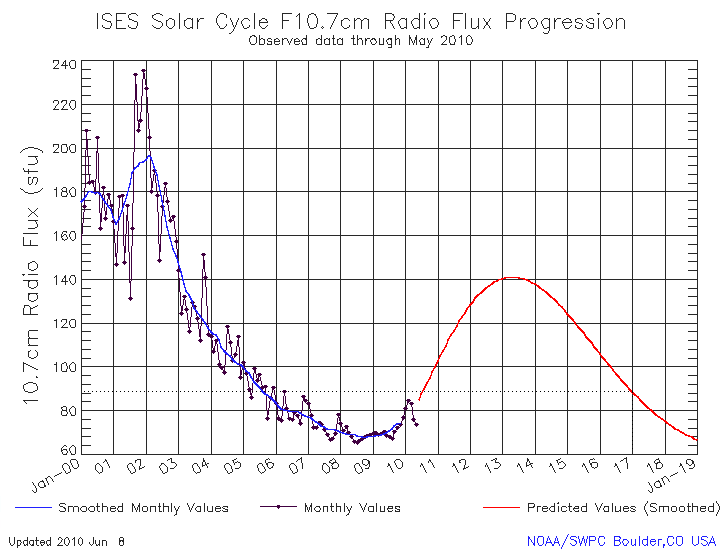
\includegraphics[width=0.6\textwidth, angle=0]{chapters/img/solarCycle.png}
\caption{Solar activity projection up to 2019. \emph{(Source: NOAA/Space Weather Prediction Center.)} }
\label{fig:f10.7}
\end{figure}

In order to provide the longest possible lifetime for the mission it is essential that the launch is timed in such a way that the satellites are in orbit most of the time during solar minimum. For this reason a launch on March 1st 2017 is planned. This also gives enough time for development and production. For further information on the timeline, please refer to section \ref{frPMgantt}.

\section{Space Segment}
\label{frSS}

This section covers the astrodynamical characteristics of the mission. The emitter orbit is covered first, then in section \ref{frSSRO}, all receiver orbits are examined. The formation and its properties are discussed in section \ref{frSSSC}. Collision avoidance is described in section \ref{frSSCA} and, finally, section \ref{frSEaS} covers the orbital environment and whether the mission is going to be heavily affected by it. 

\subsection{Emitter Orbit}
\label{frSSEOD}

\subsubsection{Orbital Parameters}
\label{frSSEODOP}

The emitter satellite is injected into a circular orbit at an altitude of 500 km. The eccentricity is frozen at 0. Inclination is chosen to be 85 degrees, as this allows access to polar areas, which are places of interest for the mission. Furthermore, the inclination provides an inherent relative phase for the crossing orbits. The \acl{RAAN} can be chosen arbitrary for the start of the mission, as no specific target is assumed for the mission. For consistency, in all following discussions it is assumed to be 0 degrees. The same goes for the Argument of Perigee and the True Anomaly. As the orbit is circular, these values are not really relevant. The emitter satellite acts as the reference for all the receiver satellites.

The orbit is non-sunsynchronous and does not have a specific repeat track. This allows for larger coverage of the Earth. 

Figure \ref{fig:confmax} on page \pageref{fig:confmax} shows the emitter satellite (labeled as Base) in Orbit 1.

A few basic properties of this orbit can be derived and are shown in table \ref{table:orb1ref} on page \pageref{table:orb1ref}. All the values were generated with the help of \cite{larson}, \cite{spacedesign} and \cite{constDesign}.

\begin{table}[!h]
\begin{centering}
\begin{tabular}{lccr}
\toprule
Parameter				&			Symbol			&			Value			&			Unit \\
\hline \hline
Altitude				&			h						&			500				&			[km]	 \\
Semi-major Axis	&			a						&			6871			&			[km]	 \\
Eccentricity		&			e						&			0				  &			[-]	 \\
\acs{RAAN}			&			$\Omega$		&			0				&			[deg]	 \\
Period (mins)		&			P						&			94.6135	&			[mins]	 \\
Revolutions per day		&									&			15.2198	&			[revs/day]	 \\
Angular Velocity		&			n						&			3.805	&			[deg/min]	 \\
Circular Velocity		&			V						&			7.6127	&			[km/s]	 \\
Max. Eclipse		&			 	$T_e$					&			35.75	&			[mins]	 \\
Node Spacing	&			 						&			23.72	&			[deg]	 \\
Node Precession	&			 $\dot{\Omega}$					&			-0.6667	&			[deg/day]	 \\
\bottomrule
\end{tabular}
\caption{Orbital properties of the emitter satellite.}
\label{table:orb1ref}
\end{centering}
\end{table}
%--------------
\subsubsection{Orbit Decay}
\label{frEmOD}
Atmospheric drag is by far the most relevant perturbation for \ac{LEO} satellites that causes loss of altitude and thus decays the orbit. It directly relates to mass as it influences the amount of fuel required to maintain the orbit, where as the mass influences the rate at which the orbit decays. Altitude selection relies heavily on estimation and analysis of drag data as for longer mission times, higher altitudes are preferred, while optical instruments prefer lower altitudes for increased accuracy.

The drag that the satellite experiences due to atmospheric density is described by the following formula:

\begin{equation}
D = -\frac{1}{2} C_D \rho V^2A
\label{drag}
\end{equation}

It follows that orbital parameter changes (semi-major axis, period and velocity respectively) per orbit are calculated using the following equations (assuming negligible eccentricity):

\begin{equation}
\Delta a = -2 \pi \left( C_D \frac{A}{m} \right) \rho a^2
\label{deltaSMA}
\end{equation}
\begin{equation}
\Delta P = -6 \pi^2 \left( C_D \frac{A}{m} \right) \rho \frac{a^2}{V}
\label{deltaP}
\end{equation}
\begin{equation}
\Delta V = \pi \left( C_D \frac{A}{m} \right) \rho aV
\label{deltaV}
\end{equation}

The fundamental problem with accurately predicting effects due to atmospheric drag is twofold: firstly it is very hard to predict the satellite's ballistic coefficient:

\begin{equation}
\frac{m}{AC_D}
\label{ball}
\end{equation}

Even with a well known mass to area ratio, the coefficient of drag can be highly variable, highly dependent on the shape of the satellite and its orientation with respect to the velocity vector. It is usually determined in laboratory conditions. For the orbit decay analysis the following equation for the coefficient of drag was used:

\begin{equation}
C_D = \alpha C_{DS} + \beta C_{DD}
\label{cd}
\end{equation}

where $C_{DS}$ is the specular coefficient of drag, $C_{DD}$ is the diffuse coefficient of drag, $\alpha$ and $\beta$ are component fractions which are determined experimentally. The specular coefficient of drag is usually predominant. In reality this drag coefficient changes. The cross-sectional area normal to the velocity vector can also vary for the swarm satellites if the whole platform is reoriented for instrument pointing. These parameters were adjusted in such a way that a final average $C_D$ of 2.22 for the emitter as well as the receiver was achieved. This is a value which is commonly used in space mission design.

The cross-sectional area of the satellite perpendicular to the velocity vector for a sample period of 6 hours can be seen in figure \ref{fig:area} on page \pageref{fig:area}. The graph was generated using the correct geometry of the satellite simulated in the Satellite Tool Kit\texttrademark software, issued by AGI, Inc. The software also computes the mean area - 1.045948 m$^2$. This will be the area used for lifetime analysis. The mass used is the final estimated satellite loaded orbit mass from section \ref{DDMBB}. It is computed to be 22.87 kg/m$^2$. This is well within the normal range for regular satellites \cite{larson}.

\begin{figure}[ht!]
\centering
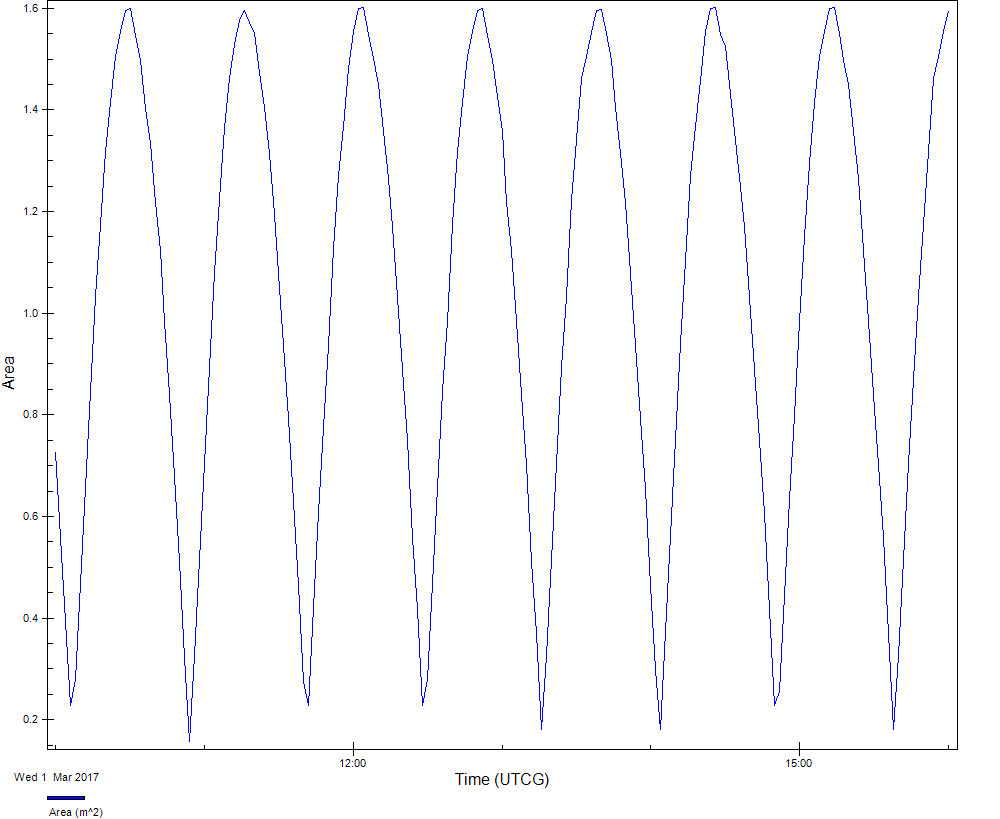
\includegraphics[width=0.4\textwidth, angle=0]{chapters/img/wetareaEmitter.png}
\caption{Simulated cross-sectional surface area of the emitter satellite perpendicular to velocity vector.}
\label{fig:area}
\end{figure}

The second reason drag calculations are so unreliable, is because air density at any altitude is highly variable. Raising air density is primarily connected with solar activity. As solar activity increases every 11 years the atmosphere heats up. Seemingly contrary to conventional gas laws that would dictate a fall in density as the gas expands, the atmosphere simply rises, increasing density at higher altitudes. This was previously discussed in section \ref{frLSLD}.

The density difference during solar maxima and minima for different altitudes is shown in figure \ref{fig:densityProfile} on page \pageref{fig:densityProfile}. Depending on the altitude, the density could vary for up to a whole order of magnitude between the minimum and maximum.

\begin{figure}[ht]
\centering
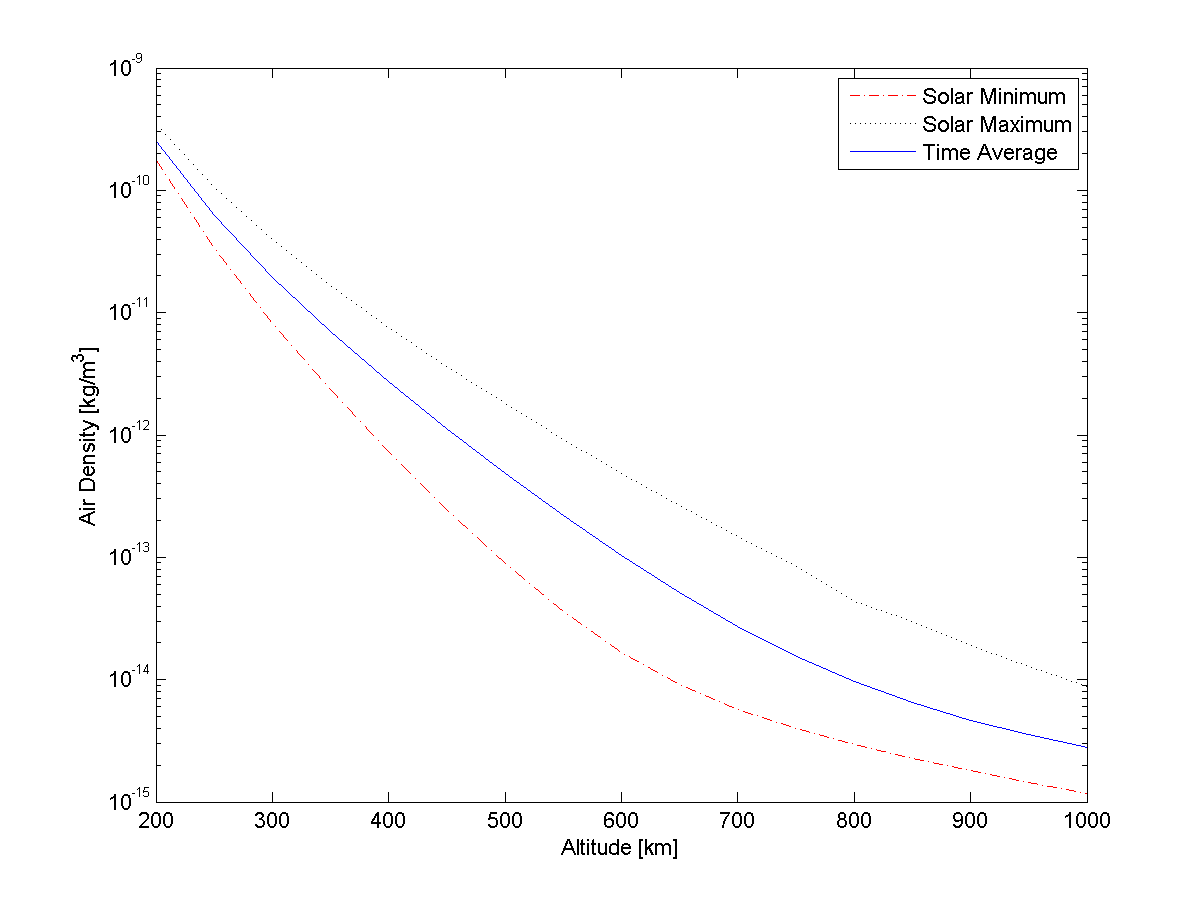
\includegraphics[width=0.5\textwidth, angle=0]{chapters/img/densityAltitude.png}
\caption{Air density vs. orbit altitude for different solar cycle stages.}
\label{fig:densityProfile}
\end{figure}

The orbit lifetime simulation was produced using the software package Satellite Tool Kit\texttrademark and can be seen in figure \ref{fig:emLife} on page \pageref{fig:emLife}.

The simulation performs orbit propagation up to the $J_4$ factor and uses the MSIS-86 Thermospheric Model for atmospheric density calculation. In addition it takes into account solar radiation pressure with an average sun exposed area of 0.84 (this area is also estimated from the satellite model simulations).

It is obvious from the previous figure that, unmaintained, the orbit would totally decay in 4.8 years. Another notable time is the point at which the emitter passes the 450 km altitude. This occurs at approximately 3.4 years after mission start. This is the altitude that will be considered as the absolute floor and will be used to approximate the altitude of the secondary satellite orbits.

\subsubsection{Estimation of $\Delta V$}
\label{frEmDV}

In order to properly estimate the mass of the propellant required for the mission all maneuvers have to be taken into account. Every maneuver requires a certain velocity change in a specified direction. During its mission, the emitter satellite will perform the following maneuvers:

\begin{itemize}
	\item A phase change slowdown. As the satellite was released from the booster vehicle, it was injected into a drift orbit in order to separate into a certain phase shift. Once this phase shift is achieved, the satellite needs to perform a boost to bring itself back into the circular orbit. This $\Delta V$ is equal and opposite to the $\Delta V$ induced by the release mechanism. This $\Delta V$ is calculated using the following equation:
	
		\begin{equation} 
 			\omega _{drift} = (1080)\frac{\Delta V}{V} 
		\end{equation}
	where $\omega _{drift}$ is the drift rate given in deg/orbit. For the emitter to return out of its drift orbit in 90 degrees, this maneuver requires a $\Delta V$ of 64.8 m/s.
	\item A boost to change the altitude from 450 km to 500 km after approximately 3.4 years in orbit. This maneuver is performed using a simple Hohmann transfer orbit and will require two burns. A simple transfer calculation is completed using the following method \cite{spacedesign}:
	\begin{equation} 
 			V_{450} = \sqrt{\frac{GM}{a_{450}}} =  7.6405\ km/s
		\end{equation}
		\begin{equation} 
 			V_{500} = \sqrt{\frac{GM}{a_{500}}} = 7.6127\ km/s
		\end{equation}
		\begin{equation}
			a_{ellipse} = \frac{a_{500}+a_{450}}{2} = 6853\ km
		\end{equation}
		\begin{equation} 
 			V_{p} = \sqrt{\frac{2GM}{a_{450}}-\frac{GM}{a_{ellipse}}} = 7.6544\ km/s
		\end{equation}
		\begin{equation} 
 			V_{a} = \sqrt{\frac{2GM}{a_{500}}-\frac{GM}{a_{ellipse}}} = 7.5988\ km/s
		\end{equation}
			\begin{equation}
			\Delta V_1 = 1000(V_p - V_{450}) = 13.9237\ m/s
		\end{equation}
		\begin{equation}
			\Delta V_2 = 1000(V_{500} - V_a) = 13.8984\ m/s
		\end{equation}
		\begin{equation}
			\Delta V = \Delta V_1 + \Delta V_2 = 27.8221\ m/s
		\end{equation}
		
		Thus the required $\Delta V$ for the Hohmann transfer is 27.8 m/s.
	\item A deorbit burn to take the satellite down to comply with sustainability requirements. This $\Delta V$ is approximated by the following equation \cite{constDesign}:
	
	\begin{equation}
			\Delta V_{deorbit} \approx V \left[ \frac{0.5(H_i - H_e)}{2R_E + H_i + H_e} \right]
		\end{equation}
	where $H_i$ is the initial altitude, $H_e$ is the reentry altitude and $R_e$ is the Earth's radius. Using the initial altitude of 500 km and a reentry altitude of 50 km, the $\Delta V$ is calculated to be 128.73 m/s. This is a very large value and in reality can be scaled down by considering a lower initial altitude (500 km is asumed in this analysis due to the consideration that a satellite might become disfunctional at the beginning at the mission and would need to be brought down) and a higher final reentry altitude (which is arbitrary). 
	
	\item The final consideration is the orbit injection accuracy of the Soyuz launch vehicle. The manufacturer states an inclination accuracy of 0.033 degrees for a 1000 km altitude orbit \cite{soyuzman}. For the purposes of this analysis, an accuracy of 0.03 degrees is used. The following equation is used to estimate the $\Delta V$ needed to correct this error:
	\begin{equation}
			\Delta V_{plane change} = 2V_i sin \frac{\alpha}{2}
		\end{equation}
	  where $V_i$ is the initial orbital velocity. The final $\Delta V$ is 3.99 m/s.
\end{itemize}

No $\Delta V$ is required for stationkeeping as the emitter will be allowed to decay naturally while the receivers will have to perform relative stationkeeping. Furthermore, the Soyuz launch vehicle can have a initial delivery altitude error. This is not considered, since it is assumed that as long as the constellation is delivered to the same altitude, no correction will be required and the lifetime of the mission will not be jeopardized. 

The total $\Delta V$ required for the emitter is calculated to be approximately 225.38 m/s.



%-------------

\subsection{Receiver Orbits}
\label{frSSRO}

\subsubsection{Orbital Parameters}
\label{frSSRODOP}

Unlike the emitter, the receiver satellites are placed in six different orbits and have to be designed to be able to handle all orbits and yet all the satellites have to have the same mass configuration at all times.

The orbits are divided into primary and secondary. The primary orbits are shown in figure \ref{fig:confmax} on page \pageref{fig:confmax}. Receiver 1 is located in Orbit 3 which has all the same orbital characteristics of Orbit 1 as described in section \ref{frSSEODOP} with the exception of its \acs{RAAN} having a value of +2.18 degrees. This is the maximum angle of separation and is derived from the requirement of a laser reflection angle of 30 degrees. Receiver 2 in Orbit 2 on the other hand has a \acs{RAAN} of -2.18 degrees. Both of these receiver satellites pass their ascending nodes at the same time as the emitter satellite. The reason for this is that the inclination of the orbits induces a relative phase between the satellites which is favorable for collision avoidance.

Receivers 3 and 4 are placed on the same orbit as the emitter. Receiver 3 travels with a positive phase offset of 2.18 degrees in front of the emitter, while the latter is trailing the emitter with the same offset. All orbital velocities and other parameters are identical to those described in section \ref{frSSEODOP}.

The secondary orbits are designated 1S, 2S and 3S, and are arranged in a similar manner while having an orbital altitude of 525 km. Receivers 1S, 2S, 3S and 4S also correspond in their arrangement to their primary counterparts.

Parameters of the secondary orbits that are different to those of the primary are shown in table \ref{table:orbsecref} on page \pageref{table:orbsecref}.

\begin{table}[ht!]
\begin{centering}
\begin{tabular}{lccr}
\toprule
Parameter				&			Symbol			&			Value			&			Unit \\
\hline \hline
Altitude				&			h						&			525			&			[km]	 \\
Semi-major Axis	&			a						&			6896			&			[km]	 \\
Period (mins)		&			P						&			95.1298	&			[mins]	 \\
Revolutions per day		&									&			15.1372	&			[revs/day]	 \\
Angular Velocity		&			n						&			3.7843	&			[deg/min]	 \\
Circular Velocity		&			V						&			7.6127	&			[km/s]	 \\
Node Spacing	&			 						&			23.85	&			[deg]	 \\
Node Precession	&			 $\dot{\Omega}$					&			-0.6584	&			[deg/day]	 \\
\bottomrule
\end{tabular}
\caption{Orbital properties of the secondary orbits (only the parameters different to those of the primary orbits are shown).}
\label{table:orbsecref}
\end{centering}
\end{table}

The initial RAANs are yet to be determined and a very complex model is required to account for differential precessions between the primary and secondary orbits. This is crucial in order for the secondary constellation to arrive in the right place with respect to the emitter. The calculations though fall out of the scope of this investigation.

\subsubsection{Orbit Decay}
\label{frRecOD}

The orbit decay analysis is done in a manner identical to that described in section \ref{frEmOD}. The final loaded mass of all the primary receiver satellites should be the same as the final orbits are established in order to decay at the same rate. The mean drag area estimated with the STK\texttrademark software is 0.3 m$^2$. The loaded mass is taken from section \ref{DDMBB}. The area exposed to the sun (for solar pressure) is calculated to be 0.25 m$^2$. The ballistic coefficient then becomes 22.40 kg/m$^2$, which is extremely close to that calculated for the emitter satellite, certainly within the margins at this point in the design. This is key to maintaining the constellation. The final design of all the satellites should ensure they decay in the closest possible manner.

The results of the decay simulation can be seen in figure \ref{fig:recLife} on page \pageref{fig:recLife}. They are virtually the same as the decay shown in figure \ref{fig:emLife}.

The decay rate of secondary satellites is shown in figure \ref{fig:recLife2} on page \pageref{fig:recLife2}. The actual altitude was iterated in order to see that the receivers would decay to 500 km in mid August 2020. In reality the secondary satellite will have to take 0.3 kg of fuel less then the primary (at the expense of less fuel available for the deorbit maneuver) as the emitter satellite would have lost 27.8 m/s worth of propellant after the Hohmann transfer back to 500 km. This will ensure the same decay rate of the secondary leg of the mission.    


\subsubsection{Estimation of $\Delta V$}
\label{frRecDV}

During the mission different receiver satellites will require different $\Delta V$. The main concern is to equalize them as the final orbits are established. The differences are only different due to different phase shifts needed and different orbital velocities.

The satellites will need to perform the following maneuvers:

\begin{itemize}
	\item A phase shift maneuver similar to the one described in section \ref{frEmDV}. For this maneuver different drift rates are required for the satellites. Receivers 1 and 2 will need a $\Delta V$ of 32.42 m/s (drift rate assumed to be half an orbit). Receiver 3 would require 31.58 m/s, but would require an entire orbit to establish its position. Receiver 4 would require a mere 0.85 m/s.
	
	The secondary orbit satellites have a different circular velocity thus also have different $\Delta V$'s. Receivers 1S and 2S require 32.37 m/s. Receiver 3S needs 31.52 m/s, and finally, Receiver 4S requires 0.84 m/s.
	\item The deorbit maneuver will require the same $\Delta V$ for all primary satellites and is also equivalent to the that of the emitter - 128.73 m/s. The secondary satellites will require 27.8 m/s less (100.93 m/s in total) as explained earlier.
	\item The correction for orbit insertion is identical for all primary satellites - 3.99 m/s (see section \ref{frEmDV}). Secondary satellites need a $\Delta V$ of 3.98 m/s. This difference is neglegible.  
\end{itemize}

The total $\Delta V$ for each receiver satellite is computed in table \ref{table:dVrec} on page \pageref{table:dVrec}.

\begin{table}[!h]
\begin{centering}
\begin{tabular}{lcccccc}
\toprule
				&			R1/R2			&			R3			&			R4		& R1S/R2S & R3S & R4S \\
\hline \hline
Phase shift				&			32.42						&			31.58		&			0.85		& 32.37 & 31.52 & 0.84	 \\
Deorbit				&			128.73						&			128.73		&			128.73		& 100.93 & 100.93 & 100.93	 \\
Inclination Correction			&			3.99						&			3.99		&			3.99		& 3.98 & 3.98 & 3.98	 \\ \hline \hline
\textbf{Total	}		&			165.14						&			164.3		&			133.57		& 137.28 & 136.43 & 105.75	 \\
\bottomrule
\end{tabular}
\caption{Total $\Delta V$ for individual receiver satellites. Values are given in m/s.}
\label{table:dVrec}
\end{centering}
\end{table}

The largest $\Delta V$ (i.e 165.14 m/s) was used for propulsion system design.

Again no numbers are specified for stationkeeping. This topic is elaborated on in section \ref{frSSStation}.

%------------------
\begin{figure}[ht!]
\centering
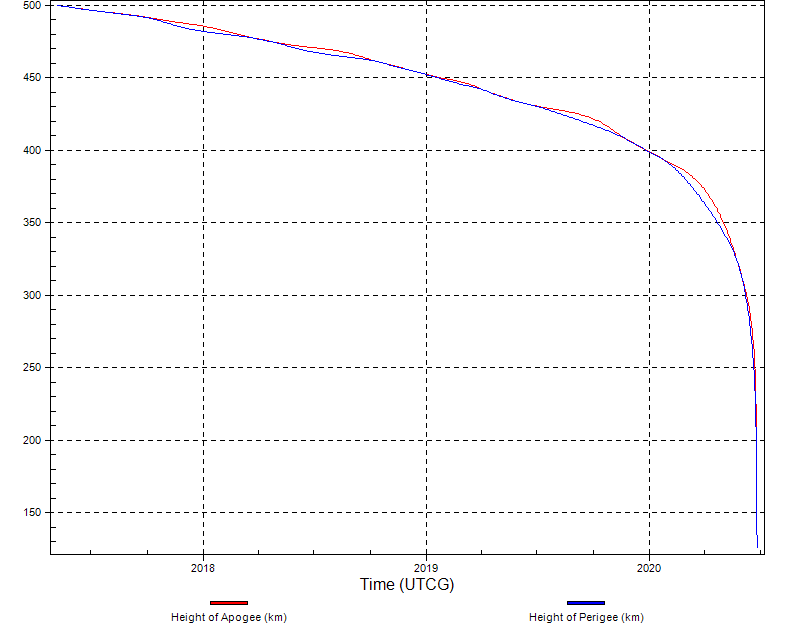
\includegraphics[width = 0.75\textwidth]{chapters/img/emitterDecay.png}
\caption{Emitter satellite orbit decay with an assumed mission start in March 2017. Values used: $C_D = 2.22$, $mass = 53.1 kg$, $area = 1.046 m^2$.}
\label{fig:emLife}
\end{figure}

\begin{figure}[ht!]
\centering
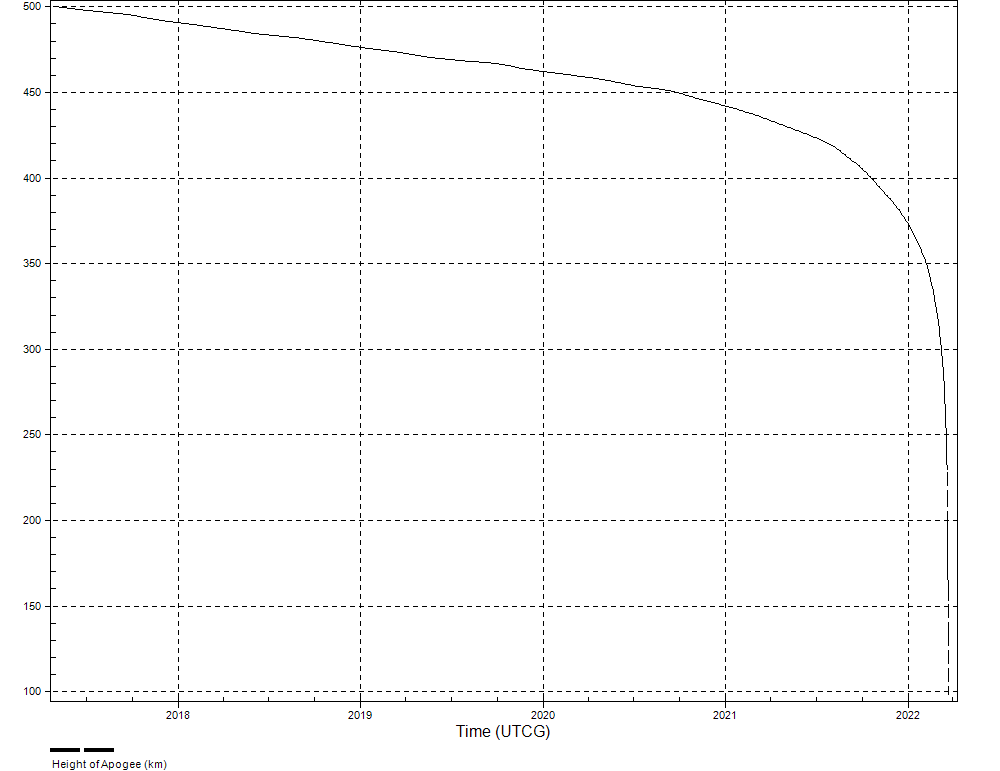
\includegraphics[width = 0.75\textwidth]{chapters/img/receiverDecay.png}
\caption{Receiver satellite orbit decay from a primary orbit with an assumed mission start in March 2017. Values used: $C_D = 2.22$, $mass = 14.92 kg$, $area = 0.3 m^2$.}
\label{fig:recLife}
\end{figure}

\begin{figure}[ht!]
\centering
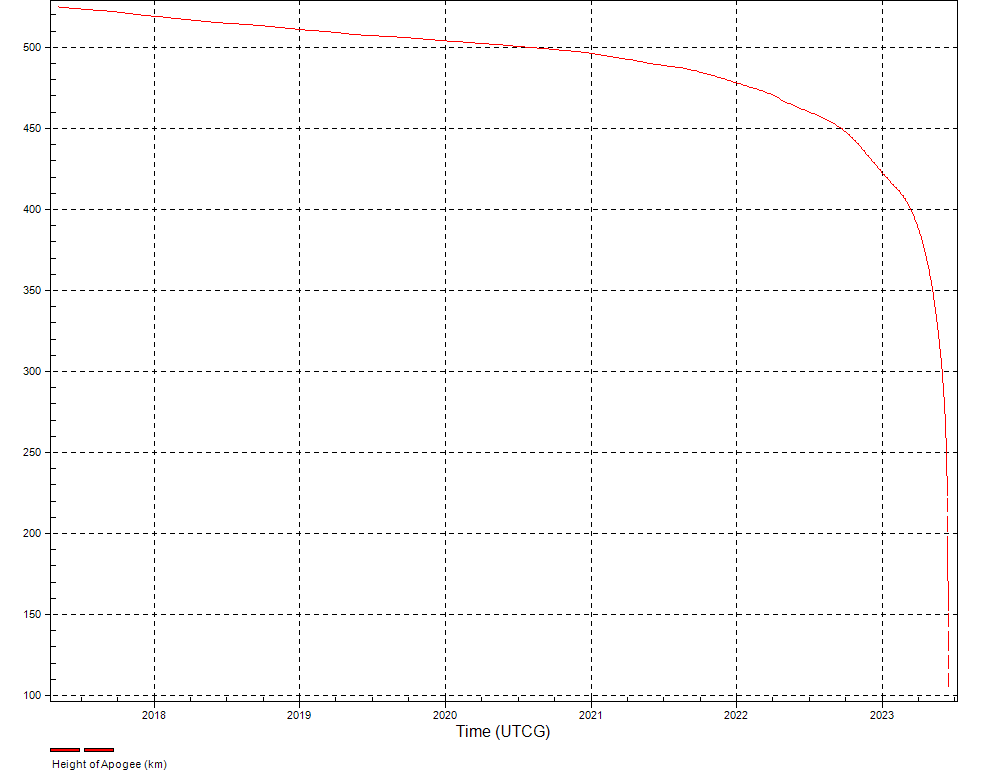
\includegraphics[width = 0.75\textwidth]{chapters/img/receiverDecay2nd.png}
\caption{Receiver satellite orbit decay from a secondary orbit with an assumed mission start in March 2017. Values used: $C_D = 2.22$, $mass = 14.92 kg$, $area = 0.3 m^2$.}
\label{fig:recLife2}
\end{figure}

\subsection{Swarm Configuration}
\label{frSSSC}

The general configuration of all the satellites has been presented in the previous section and can be reviewed in figures \ref{fig:confmax} and \ref{fig:confmin}. As explained, the general rule of separation is 2.18 degrees between the nodes of the different orbital planes and a 2.18 degree in-track phase offset for the satellites occupying the same orbit. 

\begin{figure}[!h]
\centering
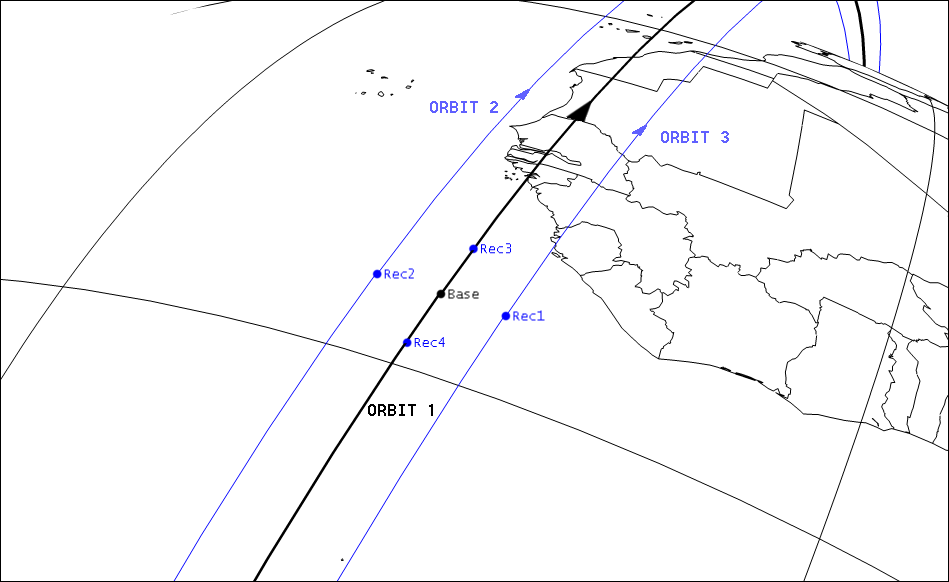
\includegraphics[width=0.8\textwidth, angle=0]{chapters/img/primaryconfmax.png}
\caption{Swarm configuration as seen when the emitter (labeled here as Base) crosses its ascending node. Orbit numbers represent the different orbital planes.}
\label{fig:confmax}
\end{figure}

\begin{figure}[!h]
\centering
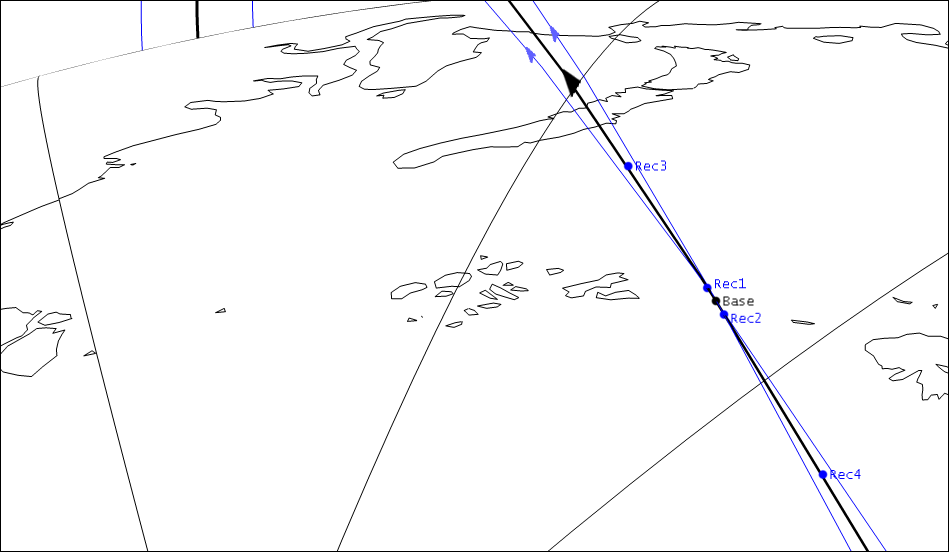
\includegraphics[width=0.8\textwidth, angle=0]{chapters/img/primaryconfmin.png}
\caption{Swarm configuration as seen when the orbit planes intersect. In this figure the intersection in ascent is pictured.}
\label{fig:confmin}
\end{figure}

A representative ground track can be seen in figure \ref{fig:ground} on page \pageref{fig:ground}.

From this general configuration several interesting parameters about the formation can be acquired. Please refer to figure \ref{fig:constgeo} for a general configuration of geometry for constellations with the same inclinations.

\begin{figure}[!h]
\centering
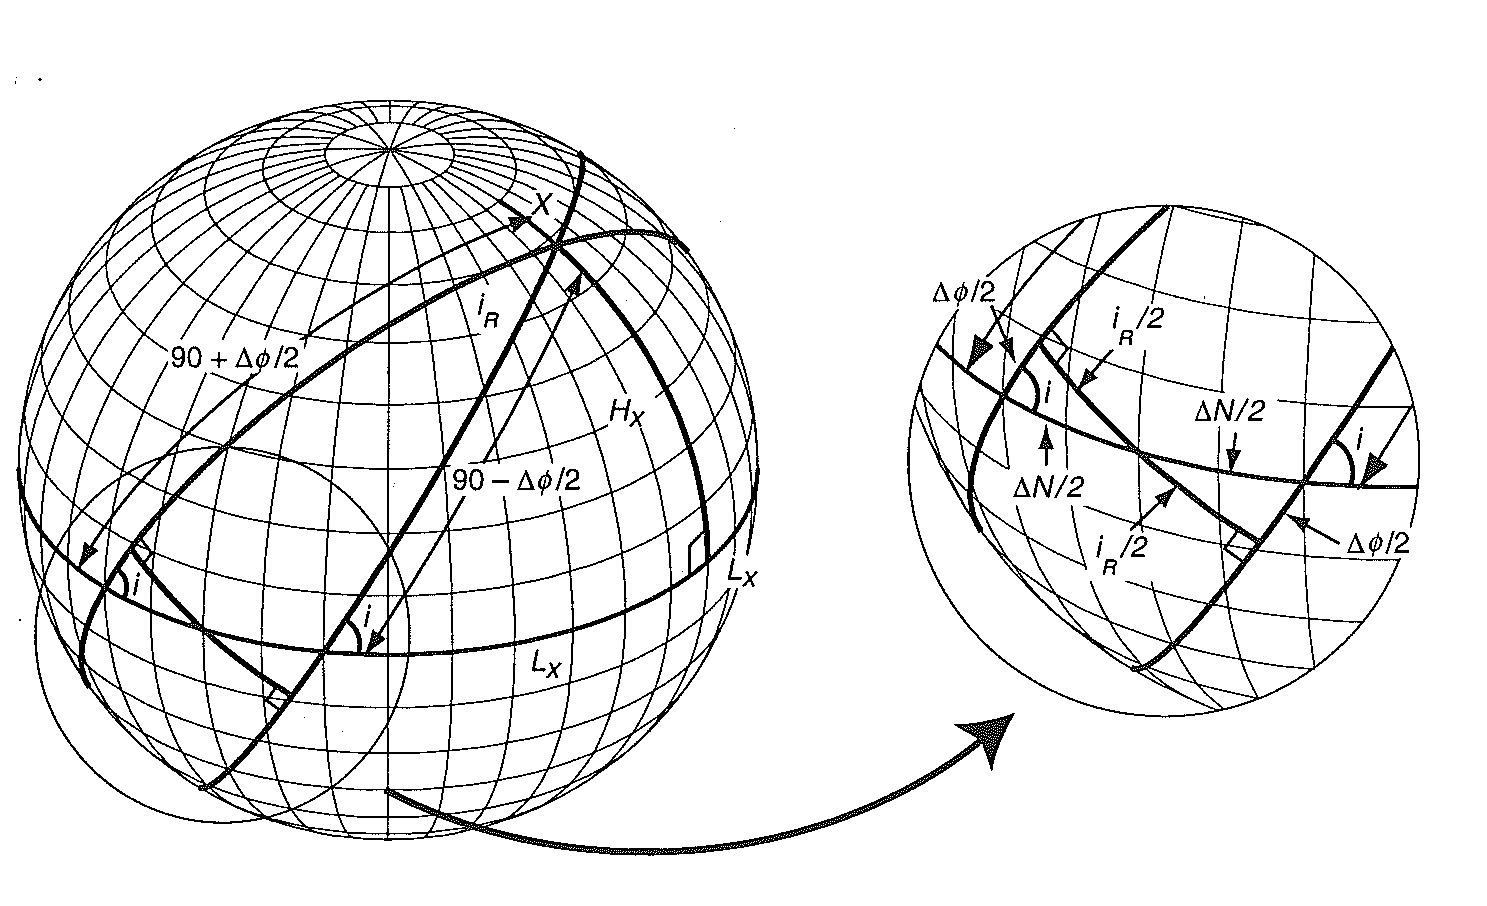
\includegraphics[width=0.8\textwidth, angle=0]{chapters/img/intersectionPhase.png}
\caption{Relative geometry between two orbital planes with the same inclination. \emph{Source: \cite{constDesign}}.}
\label{fig:constgeo}
\end{figure}

The large-scale relative motion of two satellites in different orbits is governed by only two key variables: the relative inclination, $i_R$ and relative phase, $\phi_R$. The relative inclination is the angle at which the two orbit planes intersect. The relative phase is the angle between the satellites when one intersects the other's orbit. The relative phase is the angular separation of the satellites at the time they intersect each other's orbit plane. This happens four times per orbit. The values of these angles are calculated using the following relations:

\begin{equation}
cos i_R = cos^2i+sin^2i cos \Delta N
\label{ir}
\end{equation}
\begin{equation}
\phi_R = (T_2-T_1)n+ \Delta \phi
\label{phir}
\end{equation}
where
\begin{equation}
\Delta \phi = 180 - 2 \phi
\label{deltaPhi}
\end{equation}
\begin{equation}
tan \phi = \frac{tan ( 90 - \Delta N / 2)}{cos i}
\label{tanphi}
\end{equation}

$\Delta N$ is the angular separation at the ascending nodes. Using these equations the relative inclination between Orbit 1 and 2, and 3 and 1 is 2.17 degrees; this corresponds to a separation at the nodes of 261.78 km. The relative inclination between Orbit 2 and 3 is twice this value. The relative phase between the Base and Receiver 1 is 0.1901 (or 22.82 km) as Receiver 1 always crosses Orbit 1 before the emitter satellite. Receiver 2 has the same relative phase with the emitter and trails behind on intersections. The relative phase between satellites in Orbit 2 and 3 is 0.3803 degrees or around 44.6 km.

It is also possible to calculate the maximum and minimum separation angles, $\lambda$, using the following relations:

\begin{equation}
sin ( \frac{\lambda_{min}}{2} ) = sin ( \frac{ \phi_R }{2} ) cos ( \frac{i_R}{2} )
\label{lambdamin}
\end{equation}

\begin{equation}
cos ( \frac{\lambda_{max}}{2} ) = cos ( \frac{ \phi_R }{2} ) cos ( \frac{i_R}{2} )
\label{lambdamax}
\end{equation}

The maximum and minimum angular separation between any two closest orbital planes then becomes 2.1809 and 0.1901 degrees respectively. The nadir angle can also be calculated. This is the angle between the vector pointing to any other satellite and the Earth center vector. The relations are as following:

\begin{equation}
sin (\eta_{min} ) = cos(\lambda _{max}/2) = cos(\phi _R/2)cos(i_R/2)
\end{equation}

\begin{equation}
cos(\eta_{max} ) = sin(\lambda _{min}/2) = sin(\phi _R/2)cos(i_R/2)
\end{equation}

The actual values between cross-track satellites are then 89.91 and 88.91 degrees for maximum and minimum respectively. Along-track satellites have a constant nadir angle of 88.91 degrees.

All these values are enough to simulate along and cross-track relative motion between the various satellites. Figure \ref{fig:relMotion} demonstrates the simulation of large scale relative motion between the Base, Receiver 1 and Receiver 2. Small scale motion is not simulated in this report and requires a more accurate analysis at a later point in time.

\begin{figure}
  \centering
  \subfloat[]{\label{fig:relRec1}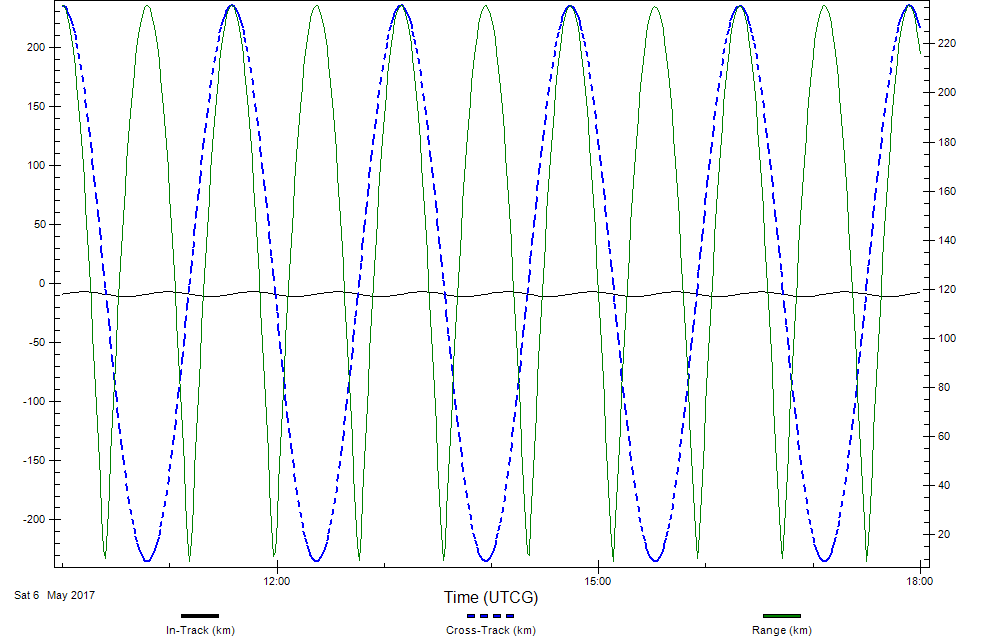
\includegraphics[width=0.9\textwidth]{chapters/img/relRec1.png}}\\                
  \subfloat[]{\label{fig:relRec2}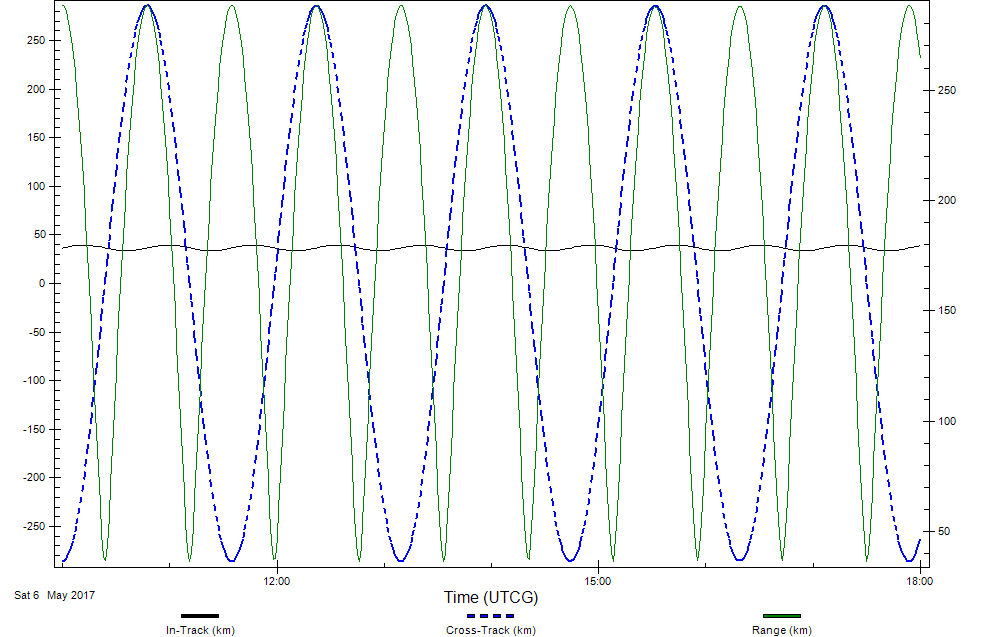
\includegraphics[width=0.9\textwidth]{chapters/img/relRec2.png}}
  \caption{Large scale relative motion (a) of Receiver 1 w.r.t. Base and (b) of Receiver 2 w.r.t. Base.}
  \label{fig:relMotion}
\end{figure}

Finally, to confirm that all orbits intersect at different points, the longitude shift $L_x$ and the latitude $H_x$ of the intersection points are computed using the following equations:

\begin{equation}
L_x = 90 - \Delta N/2
\end{equation}

\begin{equation}
tan H_x = cos\frac{\Delta N}{2}tan i
\end{equation} 

It is only interesting to see the intersections between Base, Receiver 1 and Receiver 2 as these distances are quite small (demonstrated previously to be around 22.82 km). As they all cross the ascending node at the same time the intersection of Receiver 1 will occur first at a longitude offset of 88.9096 degrees and a latitude of 85 degrees w.r.t. the node of the emitter satellite. The intersection of Receiver 2 then occurs at an offset of 91.0896 degrees w.r.t. to the emitter node. The latitude remains the same.

Since the altitude of the orbits does not affect these angles, the relations hold for orbits 1S, 2S and 3S as well.

\subsection{Stationkeeping}
\label{frSSStation}

As mentioned in section \ref{frRecDV} the satellites will not require any $\Delta V$ for stationkeeping maneuvers. This is because the concept of differential drag will be used to minimize propellant and to make the ballistic coefficients of the satellites more consistent.

The principle works in the following way: the satellites are maintained by following the slowest decaying one. This is known as relative stationkeeping. All the satellites are allowed to decay naturally in sync with that single reference. Since the orbits of every satellite are always known due to accurate navigation, it is possible to analyze decay rates. The satellites are then ordered to adjust the orientation of the solar arrays during eclipse in such a way that differential drag reinstates them into the right positions. This is further made possible due to the fact that not position acquisition but rather position knowledge (and thus correct instrument pointing) is of primary importance to data collection.

This concept has been successfully demonstrated by the ORBCOMM satellites \cite{constDesign}. It is understandable that the process of relative stationkeeping is more difficult to manage, however automated systems and prediction models can be designed to deal with this issue. Such systems however are not discussed here.  

\subsection{Collision Avoidance}
\label{frSSCA}

Collision avoidance is an integral part of formation design, yet this analysis cannot be properly performed without the detailed design of the constellation. However some design approximations can be already made to estimate the risks.

In the context of this formation, collision avoidance is important for two reasons: potential loss of two vehicles in a collision, one of them possibly being the emitter, and creation of a debris field which can jeopardize the safety of the rest of the platforms. A debris field evolution can be seen in figure \ref{fig:debris} on page \pageref{fig:debris}. This kind of debris propagation can very quickly lead to a snowball effect and destroy the whole constellation. A NASA90 debris flux model was run to simulate the propogation of a possible collision. The results can be seen in figure \ref{fig:debrisModel} on page \pageref{fig:debrisModel}. 

\begin{figure}[ht!]
  \centering
  \subfloat[]{\label{fig:elecMax}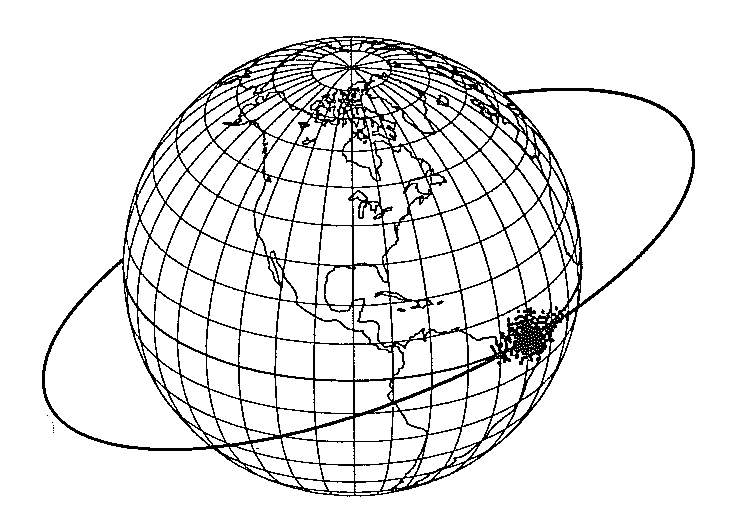
\includegraphics[width=0.4\textwidth]{chapters/img/collA.png}}                
  \subfloat[]{\label{fig:elecMin}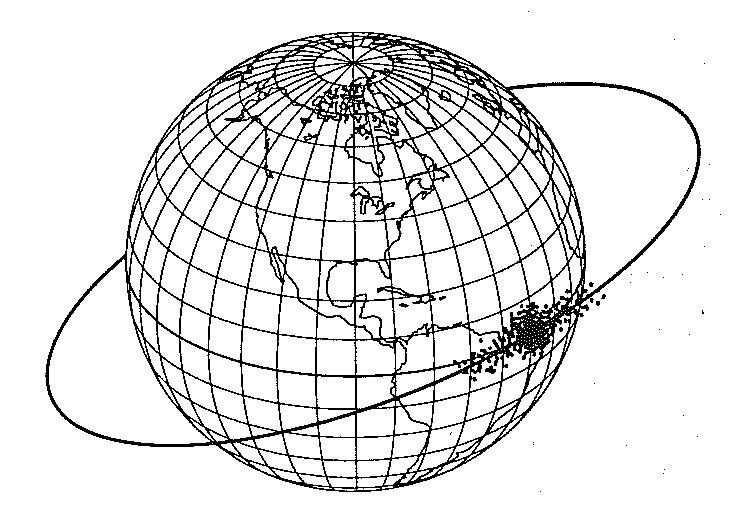
\includegraphics[width=0.4\textwidth]{chapters/img/collB.png}}\\
  \subfloat[]{\label{fig:elecMin2}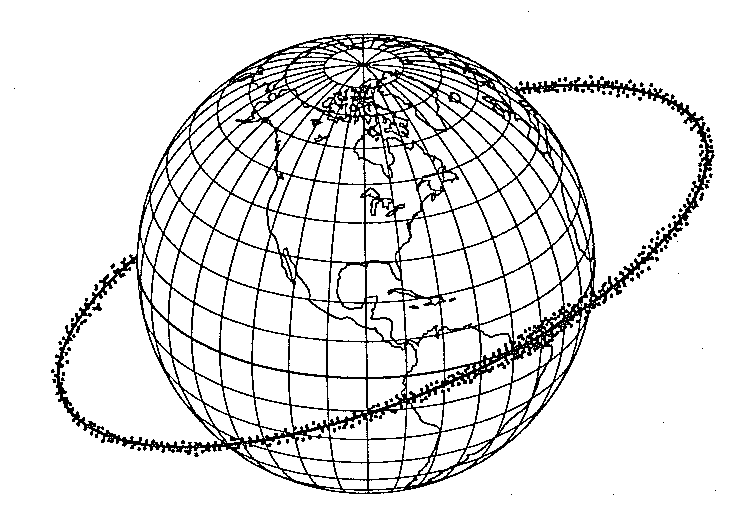
\includegraphics[width=0.4\textwidth]{chapters/img/collC.png}}
  \caption{Debris field evolution, (a) immediately after impact, (b) spreading out after some time and eventually settling into the orbit (c) and decaying. \emph{(Source: \cite{constDesign}})}
  \label{fig:debris}
\end{figure}

\begin{figure}[!h]
\centering
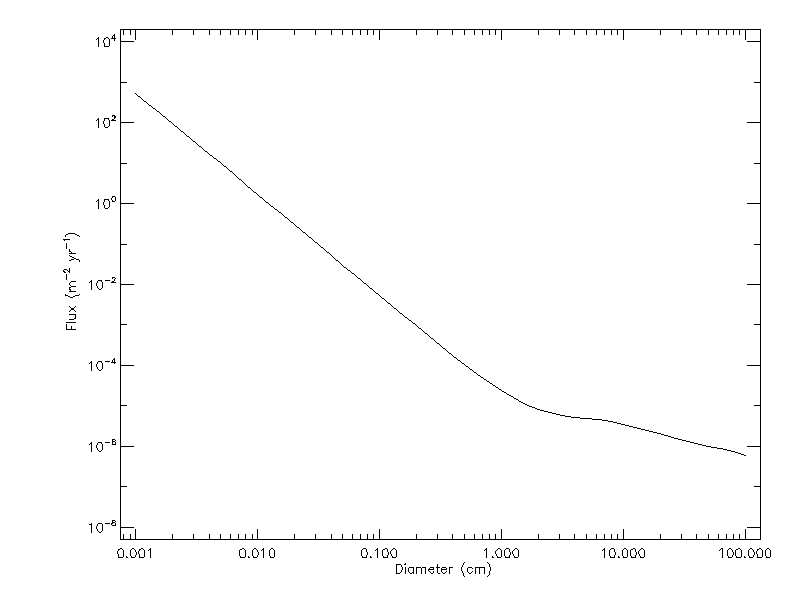
\includegraphics[width=0.5\textwidth, angle=0]{chapters/img/debris.png}
\caption{NASA90 Debris Flux simulation. Orbital altitude - 500 km, Epoch start date - May 2017. \emph{(Source: SPENVIS}.)}
\label{fig:debrisModel}
\end{figure}

Some preliminary formation collision estimates are shown in table \ref{table:coll} on page \pageref{table:coll}.

\begin{table}
	\centering
	
		\begin{tabular}{p{5cm}|p{5cm}|p{5cm}}
		\toprule
	\textbf{Parameters} & \textbf{5 Satellite Formation in 3 Planes} & \textbf{4 Satellite Formation in 3 Planes} \\
		\hline \hline
		No. of satellites & 5 & 4 \\
		No. of orbit planes & 3 & 3 \\ 
		Vertical dispersion [km] & 1 & 1 \\
		In-track dispersion [km] & 22.78 - 276 & 45.56 - 552 \\
		Potential impact area [km$^2$] & 10 & 10 \\ 
		Collision opp. per orbit & 20 & 16 \\
		Orbit period [min] & 94.62 & 95.12 \\ 
		Collision opp. per year & 1.1$*$10$^5$ & 4.0$*$10$^5$ \\
		Collision opp. in 5 years & 5.6$*$10$^5$ & 2.0$*$10$^6$ \\
		Collision prob. per opp. & 1.0$*$10$^{-7}$ & 1.0$*$10$^{-7}$ \\
		Mean number of collisions per year & 0.011 & 0.04\\
		\bottomrule
			\end{tabular}
	\caption{Inter-satellite collision estimations for a formation of 5 primary and 4 secondary satellites. Probability values based on extrapolation of values given in \cite{constDesign}.}
	\label{table:coll}
\end{table}

In order to successfully implement a safety-conscious formation design the following rules will have to be followed:
 
\begin{enumerate}
	\item Maximize spacing between platforms on orbit crossing.
	\item Remove satellites at end of life.
	\item Keep tracking the motion of "dead" satellites.
	\item Remove launcher upper stages from the orbits.
	\item Design replacement injections with collision avoidance in mind.
	\item Capture any ejected components.
	\item Avoid self-detonation.
\end{enumerate}
 
Following these rules will lead to a safer formation and eventually to an extended mission lifetime.

Another topic is collision avoidance of object that are outside the considered formation. That is with other satellites, artificial and natural bodies. Figure \ref{fig:meteor} on page \pageref{fig:meteor} demonstrates a plot of the Grun model of meteoroid flux for 500 km altitude.

\begin{figure}[ht!]
\centering
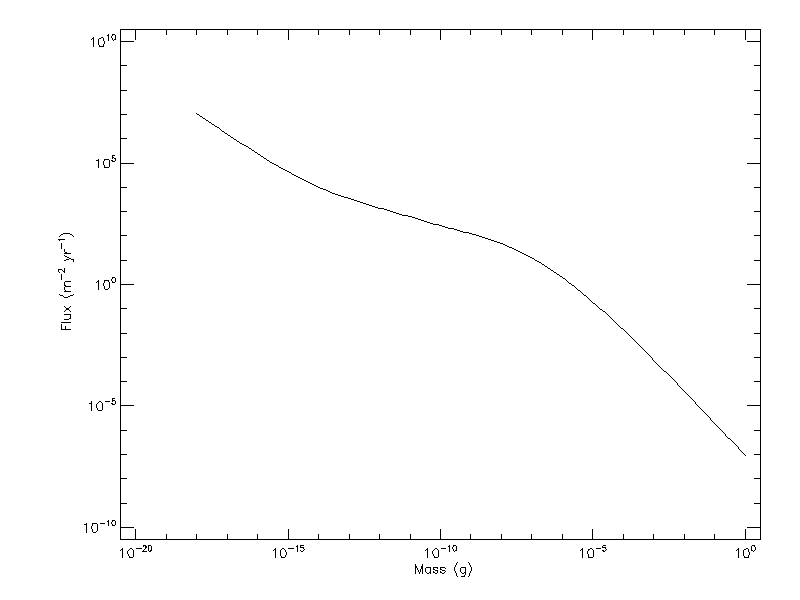
\includegraphics[width = 0.5\textwidth]{chapters/img/meteoroid.png}
\caption{Grun model meteoroid flux for an orbit of 500 km altitude. \emph{Source: SPENVIS}. }
\label{fig:meteor}
\end{figure}

It is obvious that the constellation faces quite a challenge as the low mass of the satellites makes them quite susceptible to objects with a mass of over 1 gram. It is also a problem because only pieces of about 10 cm across and more can be effectively tracked from Earth.

Pending further investigation it is not unreasonable to allow a safety margin of 5\% on the total $\Delta V$ of both satellites. This however is something better left for further investigation.

\section{Space Environment and Shielding}
\label{frSEaS}

In space, satellites are exposed to streams of highly energetic charged particles coming from the sun. Radiation from these particles can cause severe damage to satellite subsystems, including the payload. The main particle radiation source encountered by the swarm in the \ac{LEO} comes from the Van Allen Belts. These are regions around the Earth where charged particles (protons, electrons and ions) are trapped inside the magnetic field of the planet.

The total radiation dose consists of three components: proton dose, electron dose and the so-called Brehmsstrahlung X-Ray dose produced by the interaction between the electrons and the shielding material of the satellite. In \ac{LEO}, energetic protons in the inner radiation belt contribute most to the total radiation dose. This total is also strongly linked to the orbital altitude and below 1000 km will increase at approximately by the 5\textsuperscript{th} power of the altitude. Furthermore, just like with atmospheric drag, the solar activity plays a major role, thus all cases will be examined.

The number of particles trapped in the Van Allen belts in the vicinity of the orbit under question can be modeled using The Space Environment Information System (SPENVIS) that can be located at the following address: \emph{http://www.spenvis.oma.be/}. SPENVIS contains a large array of NASA and ESA (as well as other) tools and models for complex orbit analysis. For the purposes of this evaluation two models are used: AP-8 and AE-8. The first model predicts proton flux with energy levels above 100 MeV. The latter estimates the flux of electrons with energy levels of 0.5 MeV or above.

Figure \ref{fig:elecFlux} on page \pageref{fig:elecFlux} illustrates the trapped proton and electron flux as a function of distance from Earth Center. For the considered altitudes of 300 to 525 km (1.047 to 1.078 Earth radii) the satellites would encounter relatively the same order of magnitude of proton radiation. The electron radiation will decrease as the satellites decay.

It is further possible to estimate the total dose of radiation that the satellites will experience with an assumed aluminum thickness of 1mm. Another SPENVIS model, called SHIELDOSE-2, is used for this estimation. The results are presented in figure \ref{fig:dose}.

From the figure it is seen that with the standard cubesat shielding of 1 mm the total mission exposure is approximately in the order of $10^4$ rad. This is an acceptable range for all space rated instruments considered in this design (Source: \cite{larson}). However if new technologies cannot withstand this dose, an increase of thickness to 1.5 mm would bring the total dose to $10^3$ rad. 

\begin{figure}[!h]
\centering
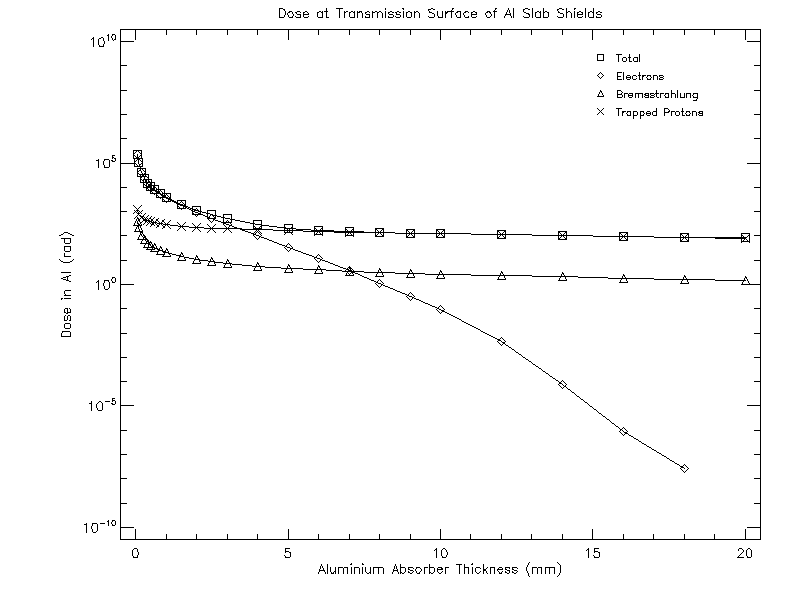
\includegraphics[width = \textwidth]{chapters/img/sd2_dose.png}
\caption{Total radiation dose based on a five year mission at a 500 km altitude. \emph{Source: SPENVIS}. }
\label{fig:dose}
\end{figure}

\begin{figure}
  \centering
  \subfloat[]{\label{fig:elecMax2}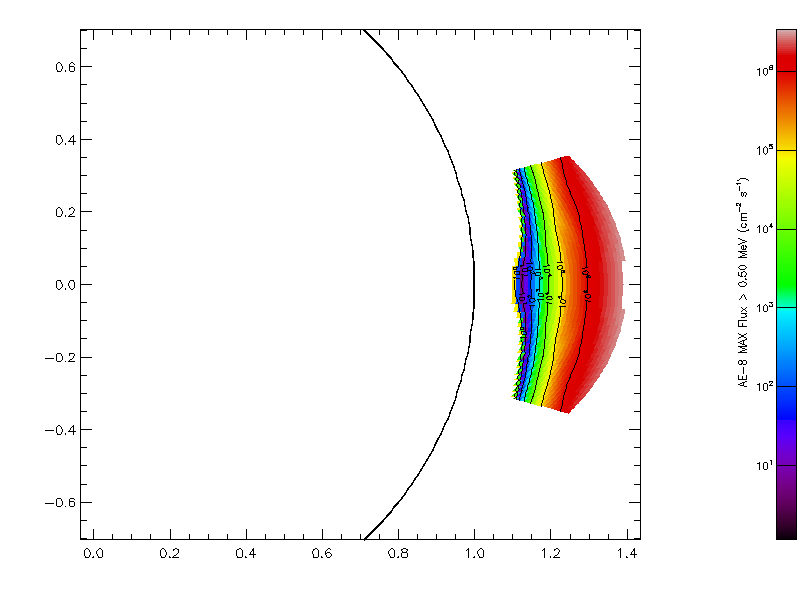
\includegraphics[width=0.7\textwidth]{chapters/img/elecFluxMax.png}}\\                
  \subfloat[]{\label{fig:elecMin3}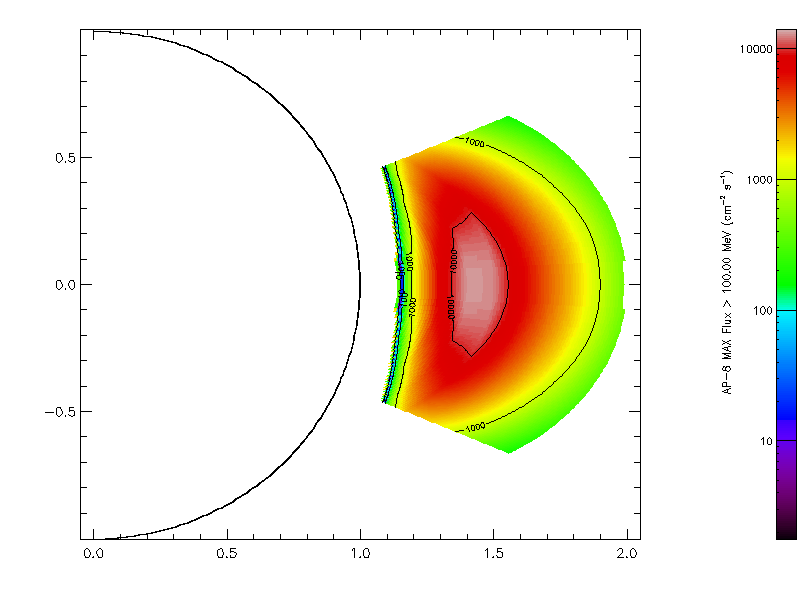
\includegraphics[width=0.7\textwidth]{chapters/img/protFluxMax.png}}
  \caption{AE-8 Electron Flux Model (energy $>$ 0.5 MeV) (a) and AP-8 Proton Flux Model (energy $>$ 100 MeV)(b).}
  \label{fig:elecFlux}
\end{figure}
 